\documentclass[preprint,12pt]{elsarticle}
\usepackage{amsmath}
\usepackage{amssymb}
\usepackage{booktabs}
\usepackage{float}
\usepackage{graphicx}
\usepackage{url}
\usepackage[hidelinks]{hyperref}
\emergencystretch=3em

\journal{Integration, the VLSI Journal}
\biboptions{numbers,sort&compress}

\begin{document}

\begin{frontmatter}

\title{SPICE-Efficient Candidate Screening and Corner-Support Calibration for GF180MCU Standard-Cell Exploration}

\author[aff1]{Jiaqing Chen\corref{cor1}}
\ead{Jq_Chen0715@buaa.edu.cn}

\author[aff1]{Feng Shao}
\cortext[cor1]{Corresponding author.}

\affiliation[aff1]{
organization={School of Integrated Circuit Science and Engineering, Beihang University},
addressline={No. 37 Xueyuan Road, Haidian District},
city={Beijing},
postcode={100191},
country={China}}

\begin{abstract}
Early standard-cell sizing and operating-condition exploration can require many transistor-level simulations before promising candidates are selected for detailed characterization. This paper presents a SPICE-efficient, provenance-aware screening and calibration workflow for GF180MCU standard-cell exploration. Two independently sampled ngspice datasets are generated for controlled INV, NAND2, NOR2, and XOR2 arcs: a 320-row primary dataset and a 480-row validation dataset, both with per-row netlist, log, model-file, status, and fidelity provenance. The evaluation combines strong tabular baselines, paired statistical tests, ranking metrics, split conformal prediction intervals, feature-importance analysis, and measured simulator/model runtime. Across 20 stratified primary-dataset splits, CatBoost gives the strongest delay model with median $R^2=0.9163$ and MAE = 0.0347 ns, while Gaussian-process regression gives the strongest power model with median $R^2=0.9992$ and MAE = 0.0559 $\mu$W. Direct primary-to-validation testing reaches $R^2=0.9187$ for delay and $R^2=0.9994$ for power. Validation-set ranking achieves Spearman correlation 0.9870 and NDCG@20\% = 0.9984, and conformal intervals provide about 94\% empirical coverage for nominal 90\% intervals. The main failure mode is zero-shot delay extrapolation to unseen process corners; adding 48 same-corner support rows raises ff-corner delay $R^2$ from 0.1645 to 0.8167. The workflow is positioned as an early-stage candidate-screening and calibration aid, not as a replacement for sign-off SPICE, layout-parasitic extraction, or full Liberty characterization.
\end{abstract}

\begin{highlights}
\item A GF180MCU/ngspice workflow supports SPICE-efficient standard-cell candidate screening.
\item Two independently sampled SPICE datasets contain 320 primary and 480 validation rows.
\item Strong tabular baselines, statistical tests, ranking metrics, and conformal intervals are reported.
\item Validation-set ranking achieves Spearman 0.9870 and NDCG@20\% = 0.9984.
\item Same-corner support samples mitigate weak zero-shot delay extrapolation.
\end{highlights}

\begin{keyword}
standard cells \sep GF180MCU \sep SPICE simulation \sep cell-library characterization \sep surrogate modeling \sep conformal prediction \sep candidate screening
\end{keyword}

\end{frontmatter}

\section{Introduction}

Standard-cell design and characterization depend on transistor-level simulation because delay and power are shaped by device sizing, process corner, supply voltage, temperature, output load, input transition time, and topology-dependent internal capacitances. Even before a production-quality Liberty file is generated, early exploration can require many SPICE runs to identify candidate regions worth further characterization. This creates a practical design-automation problem: exhaustive simulation is reliable but costly, whereas sparse exploration is cheap but can miss promising regions.

Learning-based surrogates have been widely explored for circuit modeling, analog sizing, and cell-library characterization \cite{Fayazi_AI_AMS_Review_2021,Afacan_ML_AnalogRF_Review_2021,Mina_ML_AnalogIC_Review_2022,Klemme_CellLib_ML_DTCO_ICCAD_2020,Klemme_Reliability_CellLib_TCASI_2021,Tang_KnowledgeTransfer_CellLib_MEJO_2025,Ma_GNN_CellLib_Integration_2025}. However, a surrogate model is useful in this setting only if its engineering role is bounded. It should help allocate simulation budget, rank candidates, flag uncertain regions, and identify support samples for calibration. It should not be presented as a replacement for SPICE sign-off, layout-parasitic extraction, or complete Liberty characterization.

The present work therefore reframes the task as SPICE-efficient candidate screening and corner-support calibration. Instead of asking whether a generic machine-learning model can fit a small table, we ask whether a provenance-controlled SPICE dataset can support three engineering decisions: which model class is reliable enough for early ranking, which features and operating conditions dominate the prediction, and how many same-corner support samples are needed before a new corner is trusted. This framing is particularly relevant for open-source PDK flows, where netlists, model files, simulator logs, and generated datasets can be archived together for reproducibility \cite{Google_GF180MCU_PDK_GitHub,Ngspice_Manual}.

The contribution of this paper is not a new learning algorithm. The contribution is a reproducible and bounded characterization-effort-reduction workflow, supported by a stronger evidence package than a single random-split benchmark. The workflow combines GF180MCU/ngspice data generation, source-fidelity auditing, repeated model comparison, statistical testing, validation-set generalization, candidate-ranking metrics, split conformal prediction intervals, feature-importance analysis, cross-cell few-shot transfer, and same-corner support calibration. These elements are used to support a practical claim: for controlled transistor-level arcs in GF180MCU, tabular surrogates can reduce early screening effort and guide additional SPICE sampling, provided that predictions are kept inside a clearly stated validation boundary.

\section{Related work and positioning}

Machine-learning-assisted circuit design has been studied across analog, RF, mixed-signal, and digital-library settings. Reviews of analog and mixed-signal automation describe surrogate modeling, Bayesian optimization, and neural approaches for sizing and performance prediction \cite{Fayazi_AI_AMS_Review_2021,Afacan_ML_AnalogRF_Review_2021,Mina_ML_AnalogIC_Review_2022}. Bayesian and multi-fidelity optimization methods reduce simulator calls by combining surrogate predictions with acquisition policies \cite{Lyu_Bayesian_Analog_2018,Zhang_MultiFidelity_BO_DAC_2019,He_Batched_MultiFidelity_BO_TCAD_2023}. These approaches motivate the present work, but also highlight why source fidelity and validation boundaries must be explicit.

Standard-cell characterization has a more structured engineering objective than generic circuit regression. Prior work has used machine learning to accelerate cell-library characterization and design-technology co-optimization \cite{Klemme_CellLib_ML_DTCO_ICCAD_2020,Klemme_Reliability_CellLib_TCASI_2021}. Recent studies further exploit knowledge transfer and graph-based representations for cell-library characterization across arcs, PVT conditions, or aging settings \cite{Tang_KnowledgeTransfer_CellLib_MEJO_2025,Ma_GNN_CellLib_Integration_2025}. These studies target broader characterization capability than the present controlled-arc experiment. In contrast, the present paper emphasizes a small but reproducible GF180MCU/ngspice setting in which the evidence can be audited at the level of each netlist and log file.

The revised evaluation also acknowledges that model choice matters. Classical baselines such as ridge regression, random forest, support-vector regression, gradient boosting, and multilayer perceptrons are useful but incomplete. We therefore add Gaussian-process regression (GPR) \cite{Rasmussen_Williams_GPML_2006}, XGBoost \cite{Chen_XGBoost_KDD_2016}, LightGBM \cite{Ke_LightGBM_NIPS_2017}, and CatBoost \cite{Prokhorenkova_CatBoost_NeurIPS_2018}. Graph neural networks and physics-informed neural networks are not used as direct baselines because the current released dataset is a tabular operating-point dataset rather than a graph-structured netlist/layout dataset or a differentiable physics-residual formulation. This limitation is stated explicitly rather than hidden behind a weak comparison.

Finally, engineering deployment requires more than average error. Ranking metrics are needed when the surrogate is used to select candidates, and uncertainty estimates are needed when predictions guide additional simulation. The present work therefore reports Spearman correlation, Kendall's tau, precision/recall at top-$K$, NDCG@K, percentile and maximum errors, and split conformal prediction intervals \cite{Vovk_Conformal_2005,Angelopoulos_Bates_Conformal_2021}.

\section{SPICE datasets and task formulation}

\subsection{GF180MCU/ngspice data-generation flow}

All publication-eligible rows are generated using ngspice 46 and the GF180MCU primitive-device model file \texttt{sm141064.ngspice} \cite{Ngspice_Manual,GF180MCU_Model_sm141064,GF180MCU_ReadTheDocs_CustomDesign}. The local PDK checkout used for the reported simulations corresponds to commit \texttt{de3240d7529a6970437ac3344820aaae7839f215} in the Google GF180MCU open-source PDK repository \cite{Google_GF180MCU_PDK_GitHub}. Each row records the generated netlist path, ngspice log path, simulator version, model-file path, status label, and fidelity label. Rows without successful GF180MCU SPICE provenance are excluded from the main results.

The transistor-level templates cover controlled arcs for INV, NAND2, NOR2, and XOR2. NAND2 and NOR2 use tied-input transitions for a controlled two-input topology case. XOR2 holds A2 high while A1 toggles, producing one controlled input-output arc. This design is intentionally narrower than a production standard-cell library. It does not enumerate all timing arcs, input-state conditions, rise/fall lookup tables, leakage states, or layout-extracted parasitics.

Figure~\ref{fig:workflow} summarizes the workflow. The key design decision is that SPICE-generated rows form the high-fidelity evidence base, whereas legacy auxiliary rows are used only as a negative-control source-fusion audit.

\begin{figure}[H]
\centering
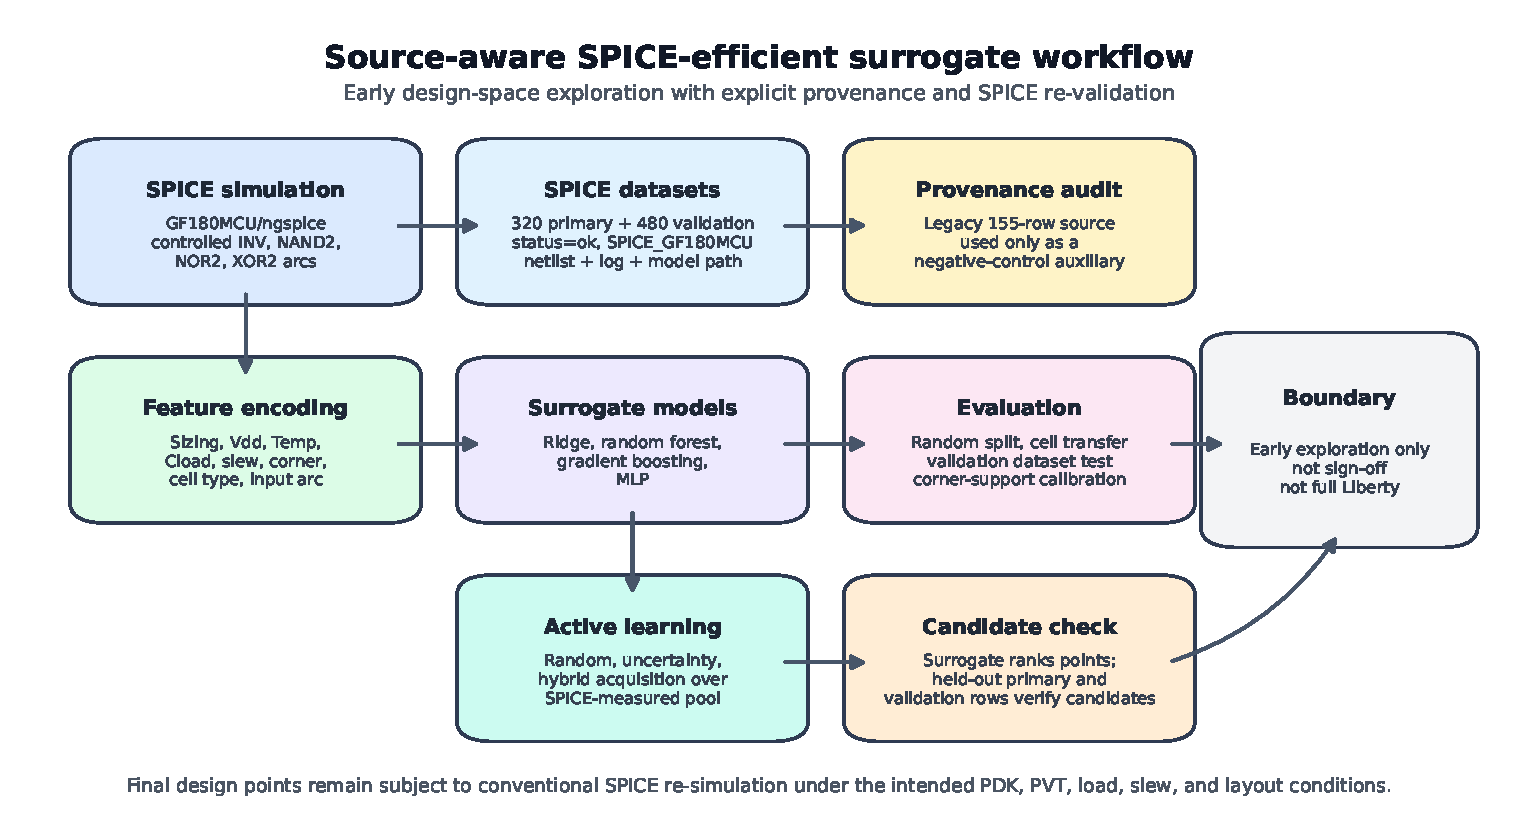
\includegraphics[width=\textwidth]{figures/fig1_workflow.pdf}
\caption{Provenance-aware SPICE-efficient screening workflow. GF180MCU/ngspice simulations generate primary and validation datasets with netlist, log, model-file, status, and fidelity metadata. Tabular surrogates are used for repeated prediction, candidate ranking, cross-cell transfer, conformal uncertainty estimation, and corner-support calibration. Final design points remain subject to SPICE re-simulation under the intended PDK, PVT, load, slew, and layout conditions.}
\label{fig:workflow}
\end{figure}

\subsection{Variables, targets, and boundary}

The input variables are NMOS width \texttt{Wn\_um}, channel length \texttt{L\_um}, PMOS/NMOS width ratio \texttt{Wp\_Wn\_ratio}, supply \texttt{Vdd}, temperature \texttt{Temp}, load capacitance \texttt{Cload\_fF}, input slew \texttt{slew\_ps}, cell type, input arc, and process corner. The targets are average propagation delay \texttt{delay\_avg\_ns} and average switching supply power \texttt{power\_avg\_uW}. Numerical variables are standardized and categorical variables are one-hot encoded with unknown-category-safe handling.

The selected channel length is fixed at 0.28 $\mu$m because this experiment uses the GF180MCU 3.3-V primitive devices and studies sizing/load/slew/corner effects rather than channel-length optimization. The process corner is incorporated through the GF180MCU model files; threshold-voltage-related device-model changes are therefore represented implicitly by the corner label and the corresponding model parameters, not by adding a separate measured $V_{\mathrm{th}}$ feature. The experiment uses a bounded temperature range from approximately -20 to 100 $^\circ$C, not the full industrial -40 to 125 $^\circ$C range. This range is sufficient for the current early-exploration validation but remains a stated boundary.

\begin{table}[H]
\centering
\caption{Datasets and variable ranges used in the revised study.}
\label{tab:datasets}
\resizebox{\textwidth}{!}{%
\begin{tabular}{lrrlll}
\toprule
Dataset & Rows & Rows/cell & Corners & Main role & Notes \\
\midrule
Primary SPICE & 320 & 80 & ff/ss/typical = 104/108/108 & Training, repeated splits, transfer, ablation & Separate netlists/logs \\
Validation SPICE & 480 & 120 & ff/ss/typical = 160/160/160 & Primary-to-validation testing and corner support & Different sampling seed \\
\midrule
Variable range & \multicolumn{5}{l}{\texttt{Wn\_um}: 0.5174--4.9905 $\mu$m; \texttt{Wp\_Wn\_ratio}: 1.5047--2.9978; \texttt{Vdd}: 1.62--1.98 V; \texttt{Temp}: -20--100 $^\circ$C; \texttt{Cload\_fF}: 1.27--99.83 fF; \texttt{slew\_ps}: 10.87--499.45 ps} \\
\bottomrule
\end{tabular}
}
\end{table}

\section{Methods}

\subsection{Model families and evaluation protocol}

The revised model set includes ridge regression, SVR with an RBF kernel, GPR, random forest, extra trees, gradient boosting, histogram gradient boosting, MLP, XGBoost, LightGBM, and CatBoost. The main repeated-split protocol uses 20 stratified 80/20 primary-dataset train/test splits. Metrics include $R^2$, MAE, RMSE, MAPE, 90th and 95th percentile absolute error, maximum absolute error, fit time, and per-row inference time. Model differences are tested using the Friedman test across repeated-split $R^2$ values and paired Wilcoxon signed-rank tests on split-wise MAE values with Holm correction.

The validation protocol trains each model on all 320 primary SPICE rows and evaluates it directly on all 480 validation SPICE rows. This is a same-flow external validation because both datasets use GF180MCU/ngspice, but they are independently sampled and stored in separate netlist/log directories. It is not cross-PDK, cross-simulator, or cross-laboratory validation.

\subsection{Candidate score and ranking metrics}

For candidate screening, delay and power are converted into a normalized composite score,
\begin{equation}
s(x)=\frac{1}{2}\frac{\hat{d}(x)-\min(\hat{d})}{\max(\hat{d})-\min(\hat{d})}
    +\frac{1}{2}\frac{\hat{p}(x)-\min(\hat{p})}{\max(\hat{p})-\min(\hat{p})},
\end{equation}
where lower score is better. The same score is computed using SPICE-measured delay and power to evaluate whether surrogate-selected rows are actually good within the measured pool. Ranking quality is reported with Spearman correlation, Kendall's tau, precision@K, recall@K, and NDCG@K. These metrics are more appropriate than point prediction error alone when the engineering task is to choose which rows should receive further SPICE attention.

\subsection{Conformal intervals and support calibration}

Split conformal prediction is used to attach calibrated intervals to gradient-boosting predictions. For each split, the primary training portion is divided into a model-training subset and a calibration subset. Absolute calibration residuals define a symmetric prediction interval around the point prediction. The nominal coverage is 90\%. The same procedure is also applied to a primary-calibrated validation-set test to evaluate interval behavior on the independently sampled validation dataset.

Corner-support calibration is evaluated on the validation dataset. For each held-out corner, the model is trained on the other two corners plus $k$ same-corner support rows, where $k=0,12,24,$ and 48. The remaining same-corner rows form the query set. This experiment tests a practical rule: if a process corner is absent from the training data, a small number of same-corner SPICE rows should be added before delay predictions are trusted.

\section{Results}

\subsection{Strong tabular baselines improve both in-domain and validation accuracy}

The expanded model comparison changes the main quantitative result. In the original lightweight benchmark, gradient boosting was the strongest delay model and an MLP was the strongest power model. With stronger tabular baselines added, CatBoost becomes the strongest delay model and GPR becomes the strongest power model. Across 20 repeated primary-dataset splits, CatBoost reaches median delay $R^2=0.9163$ and MAE = 0.0347 ns. GPR reaches median power $R^2=0.9992$ and MAE = 0.0559 $\mu$W.

The same trend persists under primary-to-validation testing. Training on the 320 primary rows and evaluating on the 480 validation rows gives CatBoost delay $R^2=0.9187$ and MAE = 0.0317 ns. GPR gives power $R^2=0.9994$ and MAE = 0.0453 $\mu$W. These results support the use of modern tabular surrogates in this constrained GF180MCU setting, while avoiding a claim that graph-based or physics-informed models have been superseded.

\begin{table}[H]
\centering
\caption{Strong tabular baselines on repeated primary splits and primary-to-validation testing. Best values are model-family results under the reported protocol, not global claims across all surrogate methods.}
\label{tab:strong-baselines}
\resizebox{\textwidth}{!}{%
\begin{tabular}{lllrrrrr}
\toprule
Protocol & Target & Model & $R^2$ & MAE & 95th abs. err. & Fit time (s) & Inference ($\mu$s/row) \\
\midrule
Repeated primary splits & Delay & CatBoost & 0.9163 & 0.0347 ns & 0.0920 ns & 0.0510 & 24.13 \\
Repeated primary splits & Delay & GPR & 0.8966 & 0.0400 ns & 0.1180 ns & 0.0472 & 22.06 \\
Repeated primary splits & Delay & XGBoost & 0.8846 & 0.0419 ns & 0.1228 ns & 0.0290 & 22.11 \\
Repeated primary splits & Power & GPR & 0.9992 & 0.0559 $\mu$W & 0.1609 $\mu$W & 0.0443 & 22.54 \\
Repeated primary splits & Power & CatBoost & 0.9890 & 0.2393 $\mu$W & 0.6198 $\mu$W & 0.0502 & 23.61 \\
Repeated primary splits & Power & MLP & 0.9819 & 0.3323 $\mu$W & 0.8521 $\mu$W & 0.0929 & 20.38 \\
\midrule
Primary $\rightarrow$ validation & Delay & CatBoost & 0.9187 & 0.0317 ns & 0.1004 ns & 0.0530 & 4.19 \\
Primary $\rightarrow$ validation & Delay & GPR & 0.9176 & 0.0380 ns & 0.1299 ns & 0.1518 & 5.99 \\
Primary $\rightarrow$ validation & Delay & XGBoost & 0.8963 & 0.0384 ns & 0.1282 ns & 0.0299 & 3.84 \\
Primary $\rightarrow$ validation & Power & GPR & 0.9994 & 0.0453 $\mu$W & 0.1385 $\mu$W & 0.0669 & 5.98 \\
Primary $\rightarrow$ validation & Power & CatBoost & 0.9902 & 0.2105 $\mu$W & 0.5885 $\mu$W & 0.0476 & 3.75 \\
Primary $\rightarrow$ validation & Power & MLP & 0.9878 & 0.2660 $\mu$W & 0.6729 $\mu$W & 0.1586 & 3.16 \\
\bottomrule
\end{tabular}
}
\end{table}

The statistical tests support these model rankings. Friedman tests reject equality across the complete model set for both delay ($p=8.18\times10^{-28}$) and power ($p=1.50\times10^{-30}$). Paired Wilcoxon tests with Holm correction show that CatBoost has significantly lower split-wise delay MAE than XGBoost, gradient boosting, LightGBM, SVR, random forest, MLP, and ridge; GPR has significantly lower split-wise power MAE than the other compared models. Figure~\ref{fig:sci-checks} summarizes the model validation, conformal coverage, feature importance, and accuracy-cost trade-off.

\begin{figure}[H]
\centering
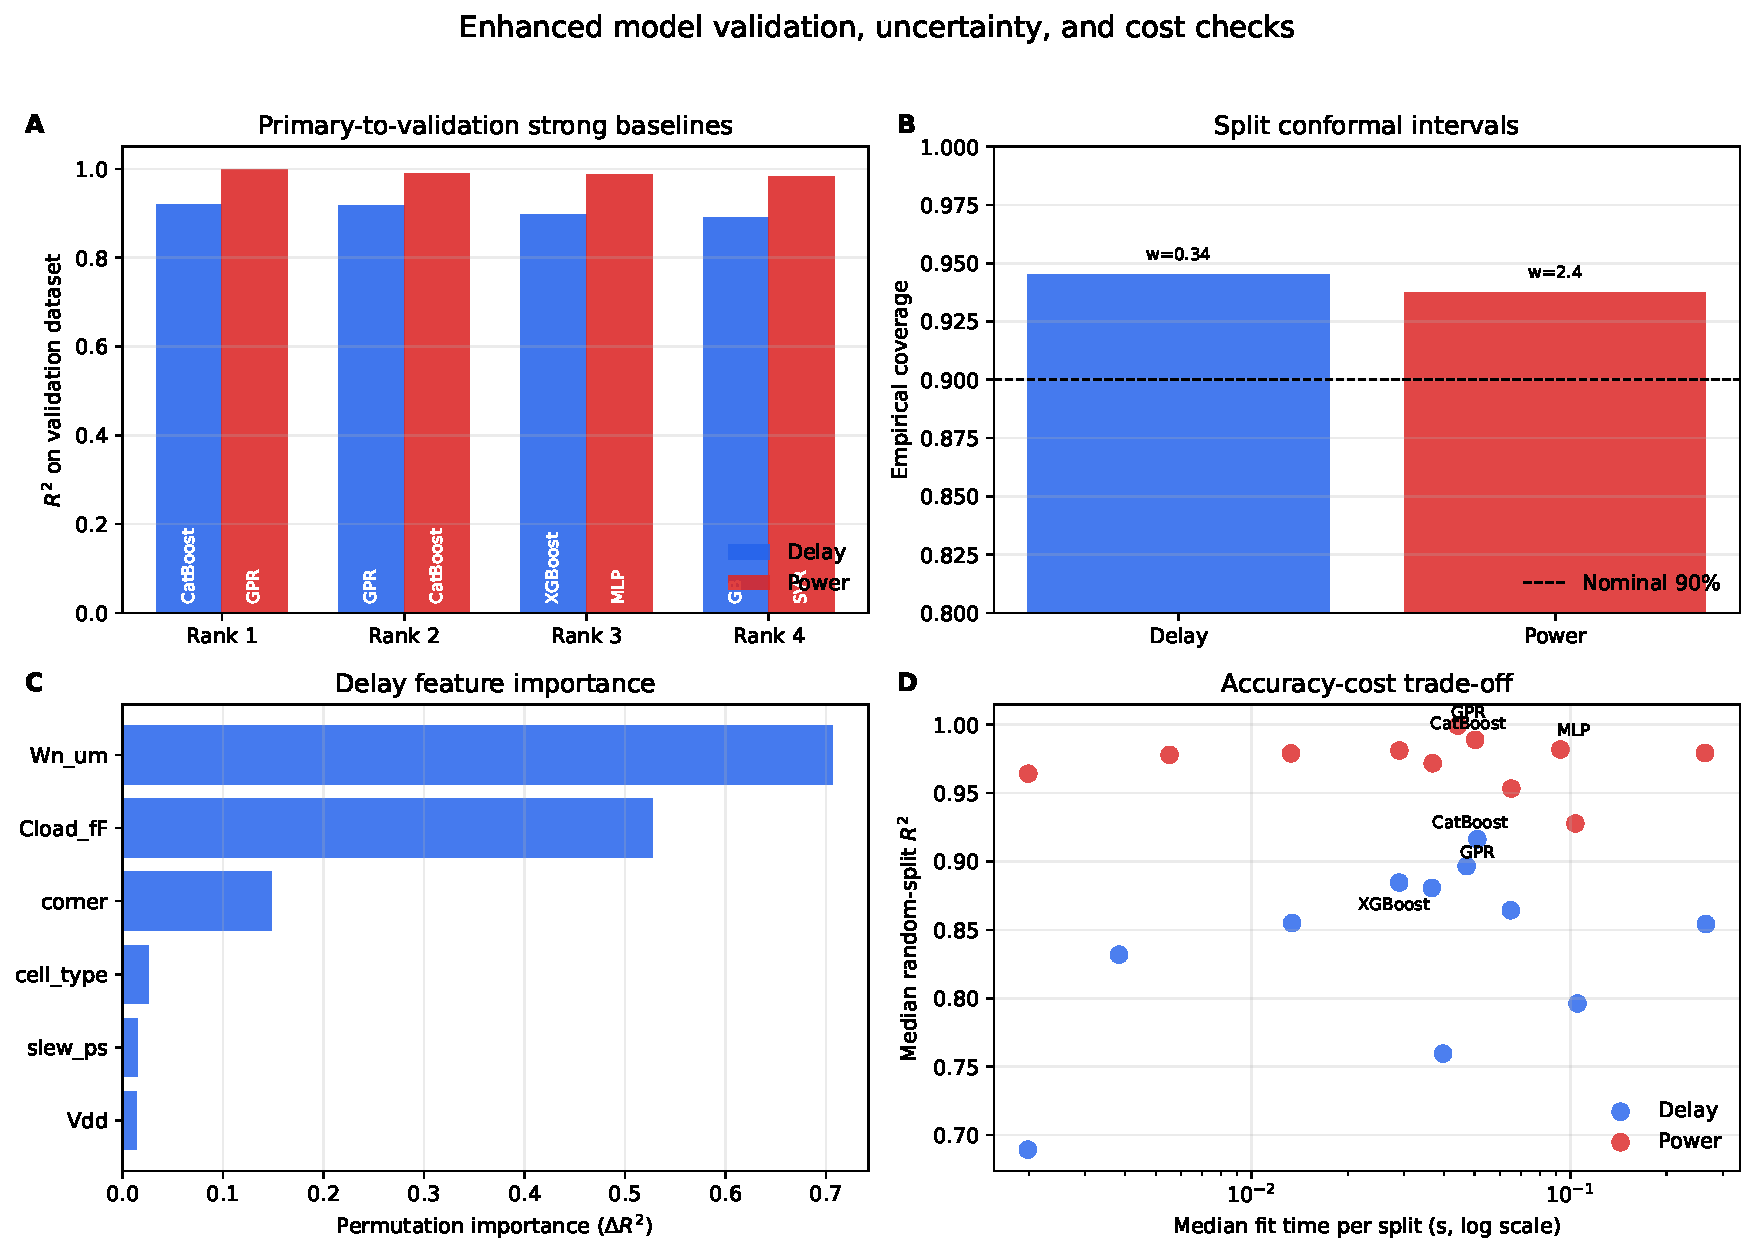
\includegraphics[width=\textwidth]{figures/fig8_sci_revision_checks.pdf}
\caption{Enhanced evaluation checks. (A) Best primary-to-validation $R^2$ values for strong tabular baselines. (B) Split conformal intervals achieve empirical coverage above the nominal 90\% level in repeated primary-dataset splits. (C) Permutation feature importance for delay prediction identifies NMOS width, load capacitance, and process corner as dominant variables. (D) Accuracy-cost trade-off across repeated primary-dataset splits, using median fit time and median $R^2$.}
\label{fig:sci-checks}
\end{figure}

\subsection{Feature importance is physically interpretable}

Permutation feature importance provides a sanity check on whether the surrogate is learning meaningful circuit behavior. For delay, the largest importance values are NMOS width, load capacitance, and process corner. This agrees with the expected dependence of propagation delay on drive strength, capacitive loading, and device speed. For power, load capacitance is dominant, followed by NMOS width, supply voltage, input arc, and cell type. Temperature has small importance for the current average switching-power target, whereas corner has substantial importance for delay but little importance for power.

The feature-ablation results support the same interpretation. Removing load and slew reduces median gradient-boosting $R^2$ from 0.8807 to 0.4184 for delay and from 0.9718 to 0.1379 for power. A sizing/PVT-only model is not sufficient, especially for power. The surrogate is therefore not simply using cell labels or width alone; load and operating variables are essential to the learned mapping.

\begin{table}[H]
\centering
\caption{Feature-ablation and permutation-importance evidence.}
\label{tab:feature-interpretation}
\resizebox{\textwidth}{!}{%
\begin{tabular}{llll}
\toprule
Question & Evidence & Result & Interpretation \\
\midrule
Are load/slew necessary? & Remove load/slew & Delay $R^2$ 0.8807 $\rightarrow$ 0.4184; power $R^2$ 0.9718 $\rightarrow$ 0.1379 & Load/slew are not optional controls \\
Are simple sizing/PVT variables enough? & Sizing/PVT-only model & Power $R^2=0.0157$ & Topology and load-related effects dominate power \\
Which variables dominate delay? & Permutation importance & Wn, Cload, corner & Consistent with drive strength, loading, and model corner \\
Which variables dominate power? & Permutation importance & Cload, Wn, Vdd, input arc & Consistent with switching-energy dependence \\
\bottomrule
\end{tabular}
}
\end{table}

\subsection{Candidate ranking is stronger than random screening}

Candidate selection is the most direct early-exploration use case. On repeated primary held-out pools, gradient-boosting ranking gives median Spearman correlation 0.9774 and Kendall's tau 0.8874 between predicted and SPICE-measured composite scores. At top-20\% selection, median precision and recall are both 0.8846. On the validation dataset, the primary-trained ranking gives Spearman correlation 0.9870, Kendall's tau 0.9031, top-20\% precision 0.9479, top-20\% recall 0.9479, and NDCG@20\% = 0.9984.

The enrichment test is also strong. When 24 validation candidates are selected by predicted score, all 24 fall inside the actual SPICE top-20\%, and all 24 also fall inside the actual SPICE top-10\%. Randomly selecting 24 validation candidates gives median top-20\% and top-10\% hit counts of 5 and 2. This result does not prove global optimization outside the sampled pool, but it does show that surrogate ranking can prioritize SPICE-measured candidates far better than random screening within the explored design space.

\begin{table}[H]
\centering
\caption{Candidate-ranking metrics for primary held-out pools and validation-set screening.}
\label{tab:ranking}
\resizebox{\textwidth}{!}{%
\begin{tabular}{lrrrrrr}
\toprule
Pool & Spearman & Kendall tau & Precision@top-10\% & Recall@top-10\% & Precision@top-20\% & NDCG@top-20\% \\
\midrule
Repeated primary held-out pools & 0.9774 & 0.8874 & 0.5385 & 1.0000 & 0.8846 & 0.9956 \\
Primary-trained validation pool & 0.9870 & 0.9031 & 0.5000 & 1.0000 & 0.9479 & 0.9984 \\
\bottomrule
\end{tabular}
}
\end{table}

\subsection{Conformal intervals quantify prediction risk}

Average accuracy is not enough for engineering decision-making, because a small number of high-error points can mislead candidate selection. Split conformal prediction provides a simple model-agnostic interval around each prediction. In repeated primary-dataset splits, nominal 90\% intervals achieve median empirical coverage of 0.9453 for delay and 0.9375 for power. The median interval widths are 0.3381 ns and 2.416 $\mu$W, respectively. When calibrated on a held-out part of the primary dataset and tested on the validation dataset, coverage remains 0.9437 for delay and 0.9396 for power.

These intervals should be interpreted as conservative screening intervals under the same GF180MCU/ngspice sampling flow. They do not guarantee coverage under cross-PDK, layout-extracted, or distribution-shifted conditions. Still, they give a practical way to identify rows whose predicted delay or power is too uncertain to trust without direct SPICE confirmation.

\subsection{Cross-cell transfer reduces few-shot target data needs}

Cross-cell transfer is evaluated with leave-one-cell-out testing. Source-cell data plus 40 target-cell support samples gives median $R^2=0.8603$ for delay and 0.9755 for power. The corresponding target-support-only baselines reach 0.5321 for delay and 0.9124 for power. At $k=20$, transfer gives an even larger delay advantage over target-only few-shot training. This indicates that source-cell data are useful in the controlled four-cell setting, but the claim should not be generalized to arbitrary sequential cells, AOI/OAI cells, or other PDKs without further validation.

\begin{figure}[H]
\centering
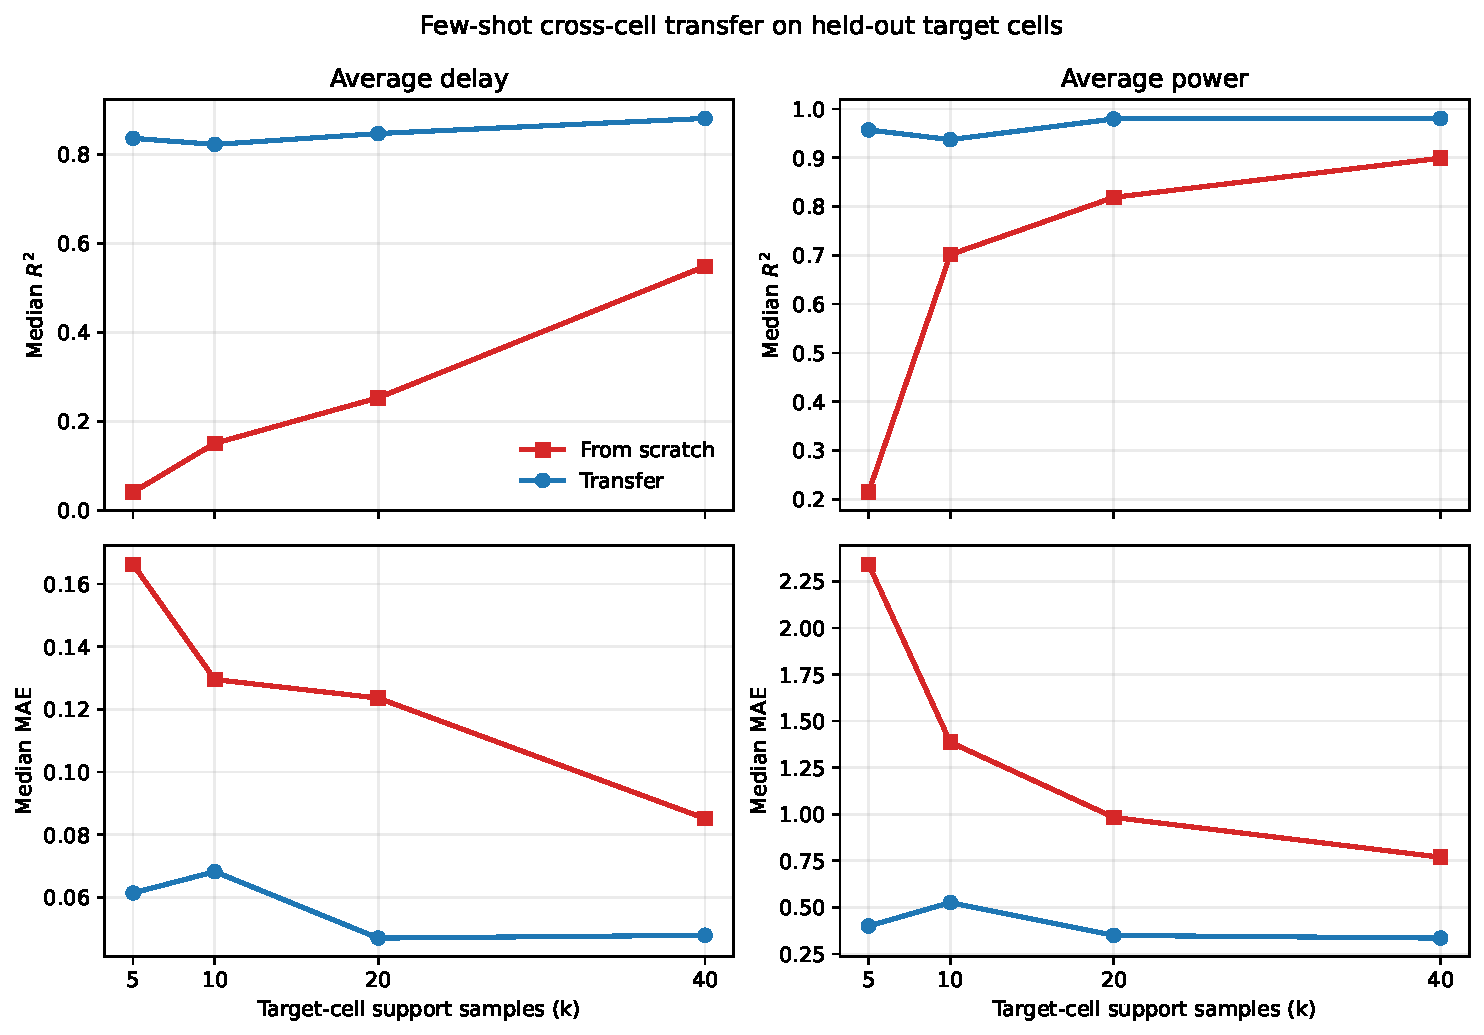
\includegraphics[width=\textwidth]{figures/fig4_fewshot_transfer_curves.pdf}
\caption{Few-shot cross-cell transfer. The transfer model uses source-cell rows plus $k$ target-cell support rows; the target-only baseline uses only the $k$ target-cell rows. Transfer is most beneficial at low support budgets and remains beneficial at $k=40$.}
\label{fig:fewshot}
\end{figure}

\subsection{Corner-support calibration converts a failure mode into a sampling rule}

The hardest stress test is not random prediction but zero-shot corner extrapolation. In the primary leave-one-corner-out test, power remains stable, but delay deteriorates sharply when the ff corner is unseen. The validation-dataset support experiment confirms the same problem and provides a remedy. With no ff support rows, median ff-delay $R^2$ is only 0.1645. Adding 12, 24, and 48 same-corner support rows raises median $R^2$ to 0.6373, 0.7641, and 0.8167. The ss corner shows a similar but less severe pattern, while typical-corner delay is easier to transfer.

The resulting operational rule is clear: a surrogate can rank and interpolate inside sampled corners, but delay predictions at a previously unseen corner should be treated as uncalibrated until same-corner SPICE support rows are added. This is a more useful conclusion than hiding the extrapolation failure, because it tells the designer where additional SPICE budget should be spent.

\begin{figure}[H]
\centering
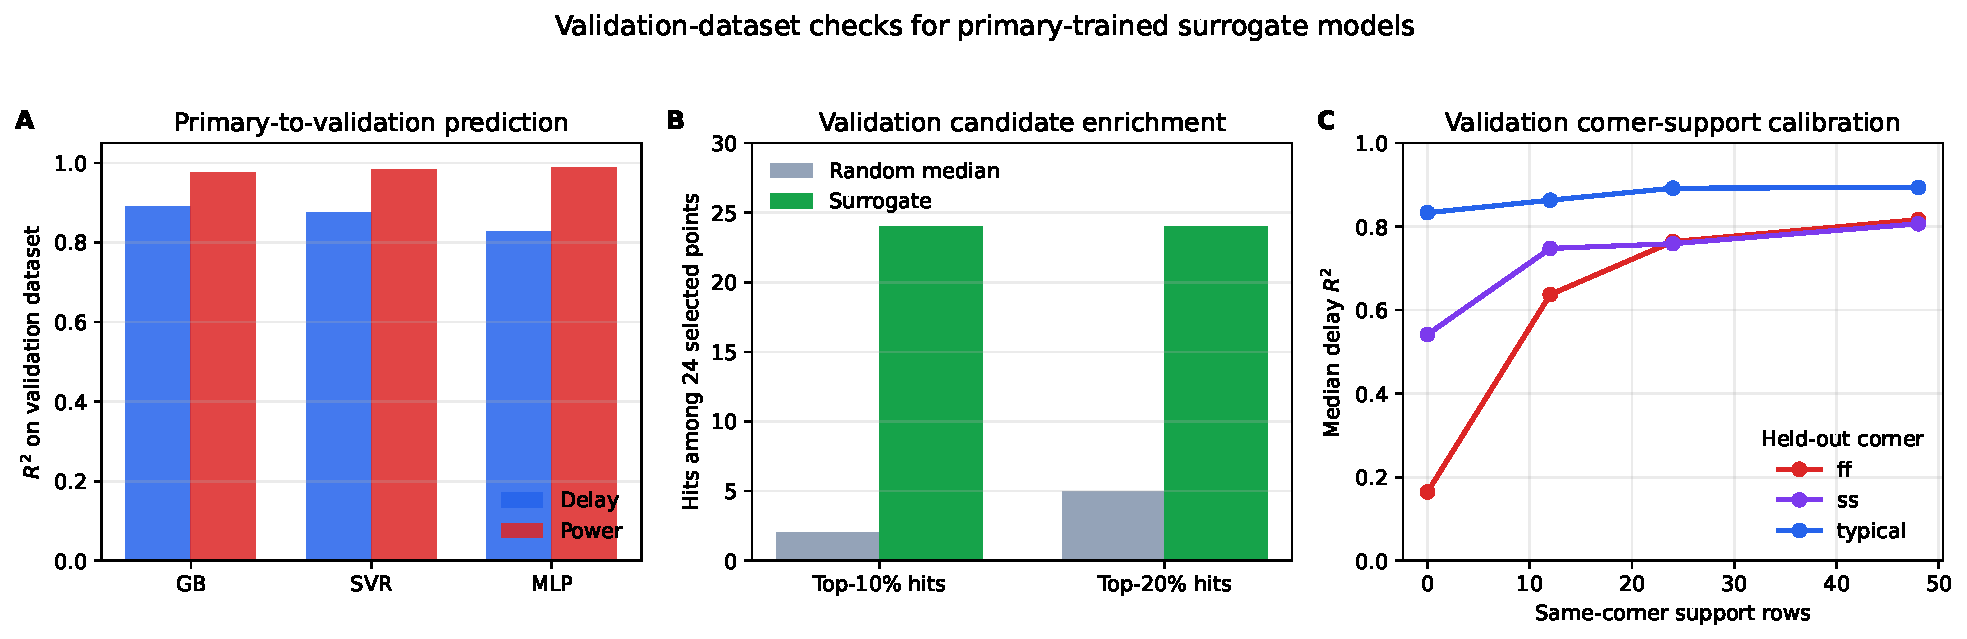
\includegraphics[width=\textwidth]{figures/fig7_validation_dataset_checks.pdf}
\caption{Validation-dataset checks. The validation set confirms primary-to-validation prediction, candidate-ranking enrichment, and same-corner support calibration. The corner-support panel shows that adding same-corner SPICE rows substantially improves held-out-corner delay prediction, especially for the ff corner.}
\label{fig:validation}
\end{figure}

\subsection{Source-fusion audit prevents unsafe use of legacy data}

The repository also contains a legacy 155-row inverter dataset. A provenance audit shows that it is not SPICE-equivalent to the primary GF180MCU/ngspice rows: it lacks the same feature set, does not include load/slew/corner coverage, and cannot be treated as a high-fidelity multi-cell source. In a reduced common-feature inverter ablation using only \texttt{Wn\_um}, \texttt{Vdd}, and \texttt{Temp}, high-fidelity-only training gives delay $R^2=0.1966$, whereas naive merging gives $R^2=-0.9201$ and a fixed 1.5x high-fidelity weighting gives $R^2=-1.3062$. Low-fidelity-only training is unusable for primary SPICE delay prediction.

This negative result is important. It shows that provenance is not merely a documentation preference; it prevents unsafe data fusion. The correct conclusion is not that a fixed source weight improves prediction, but that auxiliary rows must be validated for fidelity and feature compatibility before they enter a surrogate training set.

\section{Discussion}

\subsection{What has been strengthened}

The revised study addresses the main weaknesses of a pure ML-benchmark interpretation. Stronger tabular baselines replace the previous narrow model set. Statistical tests replace informal model-superiority claims. Ranking metrics replace anecdotal top-candidate counts. Conformal intervals provide a calibrated uncertainty layer. Parsed ngspice logs and measured model runtimes quantify simulator/model cost. Feature-importance and ablation results connect the model behavior to circuit variables. The primary-to-validation experiment tests whether the primary-trained model generalizes to newly generated SPICE rows rather than only to a random subset of the same table.

\subsection{Why delay is harder than power}

Delay prediction is more sensitive to corner and boundary conditions than average switching power in this dataset. Delay depends strongly on drive strength relative to load, process-dependent transistor current, and the local shape of the input/output transition. This is consistent with the high permutation importance of Wn, load capacitance, and corner. Average switching power is dominated by load capacitance, supply, and topology-dependent switched capacitance over the measurement window, producing a smoother target for GPR and other tabular models. The difference between delay and power accuracy therefore has a physical explanation rather than being only a model artifact.

\subsection{Cost interpretation}

The parsed SPICE logs show median elapsed times of 0.602 s for primary rows and 0.7445 s for validation rows, with XOR2 being the slowest cell type. The full primary and validation datasets represent approximately 215 s and 401 s of serial ngspice elapsed time recorded in logs. These numbers are modest because the present templates are small transistor-level controlled arcs, not complete production characterization. The practical cost reduction should therefore be interpreted at the screening level: the surrogate can rank measured or candidate rows and identify support needs before a denser SPICE sweep or full characterization flow is launched.

\subsection{Boundaries and remaining risks}

The current evidence remains bounded to GF180MCU, ngspice 46, four controlled combinational cells, and tabular operating-point features. It does not establish cross-PDK transfer to Sky130, ASAP7, FreePDK45, or commercial FinFET technologies. It does not include layout-extracted parasitics, full standard-cell height constraints, all Liberty timing arcs, leakage-state tables, or all industrial PVT conditions. It also does not demonstrate true online active learning in which new SPICE simulations are launched adaptively during the acquisition loop. The active-learning component should be read only as a retrospective pool-acquisition study.

\begin{table}[H]
\centering
\caption{Claim boundaries for the revised manuscript.}
\label{tab:boundaries}
\resizebox{\textwidth}{!}{%
\begin{tabular}{lll}
\toprule
Claim area & Supported by this work & Not established here \\
\midrule
Prediction & Repeated primary splits and primary-to-validation testing & Cross-PDK or cross-simulator accuracy \\
Candidate screening & Ranking metrics and validation-pool enrichment & Global optimization outside the sampled pool \\
Uncertainty & Split conformal intervals under same-flow sampling & Distribution-shift guarantees under new PDK/layout conditions \\
Corner use & Same-corner support improves held-out-corner delay & Reliable zero-shot delay at unseen corners \\
Cell transfer & INV/NAND2/NOR2/XOR2 controlled arcs & Sequential cells, AOI/OAI, full cell libraries \\
Data provenance & Legacy-source negative-control audit & General multi-fidelity domain adaptation \\
\bottomrule
\end{tabular}
}
\end{table}

\section{Conclusion}

This paper presents a SPICE-efficient candidate-screening and corner-support calibration workflow for GF180MCU standard-cell exploration. The workflow is based on two independently sampled ngspice datasets, explicit provenance metadata, strong tabular surrogate baselines, statistical testing, candidate-ranking metrics, conformal intervals, feature interpretation, cross-cell few-shot transfer, and validation-set corner-support calibration. The revised evidence shows that CatBoost and GPR improve the strongest delay and power results, that validation-set candidate ranking is highly enriched for SPICE top-performing points, and that weak zero-shot corner delay can be mitigated by adding same-corner SPICE support rows. The resulting claim is intentionally bounded: tabular surrogates can reduce early screening effort and guide additional simulation under a controlled GF180MCU/ngspice flow, but final design decisions still require conventional SPICE re-validation, layout-aware checks, and complete characterization under the intended design conditions.

\section*{CRediT authorship contribution statement}

Jiaqing Chen: Conceptualization, Methodology, Software, Validation, Formal analysis, Investigation, Data curation, Writing -- original draft, Visualization.

Feng Shao: Supervision, Conceptualization, Methodology, Writing -- review and editing.

\section*{Declaration of competing interest}

The authors declare that they have no known competing financial interests or personal relationships that could have appeared to influence the work reported in this paper.

\section*{Funding}

This research received no specific grant from any funding agency in the public, commercial, or not-for-profit sectors.

\section*{Data and code availability}

The primary SPICE dataset, validation SPICE dataset, SPICE-generation scripts, evaluation scripts, generated result summaries, figure-generation scripts, and SPICE netlists/logs supporting this study are available in the archived repository on Zenodo: \url{https://doi.org/10.5281/zenodo.20524583}. The live GitHub repository is available at \url{https://github.com/jqchen0715/gf180mcu-spice-surrogate-mej}.

\section*{Acknowledgments}

The authors thank the open-source PDK and ngspice communities for making publicly available tools, documentation, and process-design-kit resources that enabled the reproducible simulation workflow used in this study.

\section*{Declaration of generative AI and AI-assisted technologies in the manuscript preparation process}

During the preparation of this work, the author(s) used AI-assisted tools to support manuscript organization, language editing, code assistance, and submission-readiness checking. After using these tools, the author(s) reviewed and edited the content as needed and take full responsibility for the content of the published article.

\bibliographystyle{elsarticle-num}
\bibliography{microelectronics_journal_references}

\end{document}
